\documentclass[border=0.05in]{standalone}
\usepackage{graphicx}
\usepackage{tikz}
\usepackage{xcolor}
\usetikzlibrary{shapes.misc, patterns}

%%%%%%%%%%%%%%%%%%%%%%%%%%%%%%%%%%%%%%%%%%%%%%%%%%
%%%%%%%%%%%%%%%%%%%%%%%%%%%%%%%%%%%%%%%%%%%%%%%%%%
\begin{document}

\begin{tabular}{c c}


\begin{tikzpicture}
  \node at (0, 0) {};
  \node[draw, very thick, rounded corners] at (3.5, 0) {\Huge Speech masker};
\end{tikzpicture}
\\

\includegraphics{data_IM_pilot_v5.pdf}
&

%%% Pattern fill
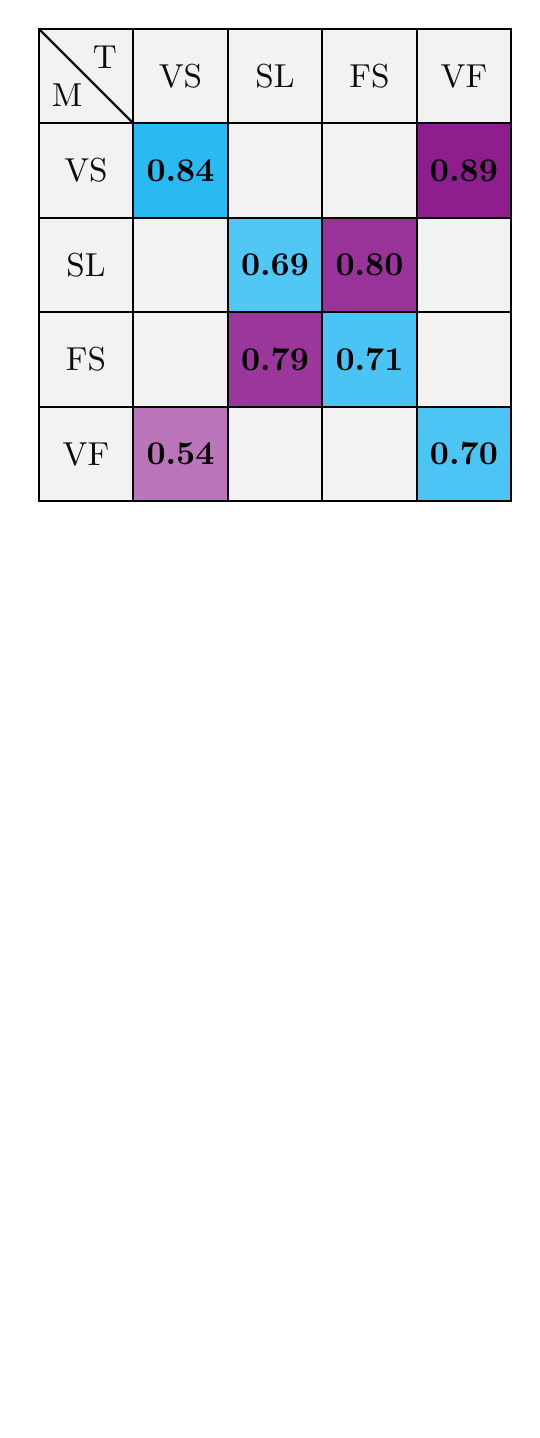
\begin{tikzpicture}[scale=1.2, every node/.style={transform shape}]
  % Target/Masker
  \node at (0.7, 11.2) {T};
  \node at (0.3, 10.8) {M};
  \draw[thick] (0, 11.5) -- (1, 10.5);
  
  % Row labels
  \node at (1.5, 11.) {VS};
  \node at (2.5, 11.) {SL};
  \node at (3.5, 11.) {FS};
  \node at (4.5, 11.) {VF};
  % Column labels
  \node at (0.5, 10.) {VS};
  \node at (0.5, 9.) {SL};
  \node at (0.5, 8.) {FS};
  \node at (0.5, 7.) {VF};
  
  % Row 1 (top)
  \draw[thick, draw=black, fill=gray, fill opacity=0.1]
     (0, 10.5) -- (0, 11.5) -- (1, 11.5) -- (1, 10.5) -- cycle;
  \draw[thick, draw=black, fill=gray, fill opacity=0.1]
     (1, 10.5) -- (1, 11.5) -- (2, 11.5) -- (2, 10.5) -- cycle;
  \draw[thick, draw=black, fill=gray, fill opacity=0.1]
     (2, 10.5) -- (2, 11.5) -- (3, 11.5) -- (3, 10.5) -- cycle;
  \draw[thick, draw=black, fill=gray, fill opacity=0.1]
     (3, 10.5) -- (3, 11.5) -- (4, 11.5) -- (4, 10.5) -- cycle;
  \draw[thick, draw=black, fill=gray, fill opacity=0.1]
     (4, 10.5) -- (4, 11.5) -- (5, 11.5) -- (5, 10.5) -- cycle;
  % Row 2
  \draw[thick, draw=black, fill=gray, fill opacity=0.1]
     (0, 9.5) -- (0, 10.5) -- (1, 10.5) -- (1, 9.5) -- cycle;
  \draw[thick, draw=black, fill=cyan, fill opacity=0.8375]
     (1, 9.5) -- (1, 10.5) -- (2, 10.5) -- (2, 9.5) -- cycle;
  \node at (1.5, 10.) {\textbf{0.84}};
  \draw[thick, draw=black, fill=gray, fill opacity=0.1]
     (2, 9.5) -- (2, 10.5) -- (3, 10.5) -- (3, 9.5) -- cycle;
  \draw[thick, draw=black, fill=gray, fill opacity=0.1]
     (3, 9.5) -- (3, 10.5) -- (4, 10.5) -- (4, 9.5) -- cycle;
  \draw[thick, draw=black, fill=violet, fill opacity=0.8875]
     (4, 9.5) -- (4, 10.5) -- (5, 10.5) -- (5, 9.5) -- cycle;
  \node at (4.5, 10.) {\textbf{0.89}};
  % Row 3
  \draw[thick, draw=black, fill=gray, fill opacity=0.1]
     (0, 8.5) -- (0, 9.5) -- (1, 9.5) -- (1, 8.5) -- cycle;
  \draw[thick, draw=black, fill=gray, fill opacity=0.1]
     (1, 8.5) -- (1, 9.5) -- (2, 9.5) -- (2, 8.5) -- cycle;
  \draw[thick, draw=black, fill=cyan, fill opacity=0.6875]
     (2, 8.5) -- (2, 9.5) -- (3, 9.5) -- (3, 8.5) -- cycle;
  \node at (2.5, 9.) {\textbf{0.69}};
  \draw[thick, draw=black, fill=violet, fill opacity=0.8]
     (3, 8.5) -- (3, 9.5) -- (4, 9.5) -- (4, 8.5) -- cycle;
  \node at (3.5, 9.) {\textbf{0.80}};
  \draw[thick, draw=black, fill=gray, fill opacity=0.1]
     (4, 8.5) -- (4, 9.5) -- (5, 9.5) -- (5, 8.5) -- cycle;
  % Row 4
  \draw[thick, draw=black, fill=gray, fill opacity=0.1]
     (0, 7.5) -- (0, 8.5) -- (1, 8.5) -- (1, 7.5) -- cycle;
  \draw[thick, draw=black, fill=gray, fill opacity=0.1]
     (1, 7.5) -- (1, 8.5) -- (2, 8.5) -- (2, 7.5) -- cycle;
  \draw[thick, draw=black, fill=violet, fill opacity=0.7875]
     (2, 7.5) -- (2, 8.5) -- (3, 8.5) -- (3, 7.5) -- cycle;
  \node at (2.5, 8.) {\textbf{0.79}};
  \draw[thick, draw=black, fill=cyan, fill opacity=0.7125]
     (3, 7.5) -- (3, 8.5) -- (4, 8.5) -- (4, 7.5) -- cycle;
  \node at (3.5, 8.) {\textbf{0.71}};
  \draw[thick, draw=black, fill=gray, fill opacity=0.1]
     (4, 7.5) -- (4, 8.5) -- (5, 8.5) -- (5, 7.5) -- cycle;
  % Row 5 (bottom)
  \draw[thick, draw=black, fill=gray, fill opacity=0.1]
     (0, 6.5) -- (0, 7.5) -- (1, 7.5) -- (1, 6.5) -- cycle;
  \draw[thick, draw=black, fill=violet, fill opacity=0.5375]
     (1, 6.5) -- (1, 7.5) -- (2, 7.5) -- (2, 6.5) -- cycle;
  \node at (1.5, 7.) {\textbf{0.54}};
  \draw[thick, draw=black, fill=gray, fill opacity=0.1]
     (2, 6.5) -- (2, 7.5) -- (3, 7.5) -- (3, 6.5) -- cycle;
  \draw[thick, draw=black, fill=gray, fill opacity=0.1]
     (3, 6.5) -- (3, 7.5) -- (4, 7.5) -- (4, 6.5) -- cycle;
  \draw[thick, draw=black, fill=cyan, fill opacity=0.7]
     (4, 6.5) -- (4, 7.5) -- (5, 7.5) -- (5, 6.5) -- cycle;
  \node at (4.5, 7.) {\textbf{0.70}};
  
  % Invisible node to force the matrix up
  \node at (0, -3) {};
\end{tikzpicture}

\end{tabular}

%%%%%%%%%%%%%%%%%%%%%%%%%%%%%%%%%%%%%%%%%%%%%%%%%%
%%%%%%%%%%%%%%%%%%%%%%%%%%%%%%%%%%%%%%%%%%%%%%%%%%
\end{document}